\documentclass[laboratorio]{guia}

\def \practnum {9}
\def \practica {Difracci\'on de la luz}

\def \materia {Laboratorio de F\'\i sica II para Qu\'\i micos}
\def \periodo {2do. Cuatrimestre de 2015}
\def \catedra {Pablo Cobelli}
\def \website {http://materias.df.uba.ar/f2qa2015c2}

\usepackage{graphics}
\usepackage{amsmath}
\usepackage{amsfonts}
\usepackage{graphicx}
\usepackage{float}
\usepackage{wrapfig}
\usepackage{subfigure}
\usepackage{bm}
\usepackage{grffile}
\usepackage{color}
\usepackage{framed}
\usepackage[utf8]{inputenc}
\usepackage[T1]{fontenc}
\usepackage{lmodern}
\usepackage{circuitikz}
\usepackage[spanish]{babel}
\usepackage{babelbib}
\selectbiblanguage{spanish}



%----------------------------------------------------------
% Agrega al path de figuras el subdirectorio con el mismo
%     nombre que el archivo principal del proyecto
\graphicspath{{./\jobname/}}

%----------------------------------------------------------
% Definicion del entorno 'sabermas'
\makeatletter
\definecolor{shadecolor}{rgb}{0.89,0.91,0.94}
\newenvironment{sabermas}[1]{%
\vfill
\begin{shaded}
  \begin{center}
  {\textsection{Para saber m\'as}}
  \end{center}
  #1
\sf } 
{%
\end{shaded}%
}
\makeatother

%----------------------------------------------------------
% Definicion del entorno 'problema'
\newcounter{ContadorProblema}
\setcounter{ContadorProblema}{0}
\newcounter{TieneFiguraAsociada}
\setcounter{TieneFiguraAsociada}{0}
\newcounter{UbicacionFigura}
\setcounter{UbicacionFigura}{0}

\newenvironment{problema}[2][]
{%
    \ifx\relax#1\relax%
        \setcounter{TieneFiguraAsociada}{0}
        \else
        \setcounter{TieneFiguraAsociada}{1}
    \fi
    \def \archivofigura {#1}
    % 
    \refstepcounter{ContadorProblema}
    \noindent%
    \ifnum\value{TieneFiguraAsociada} < 1%
        {\sffamily \bfseries Problema \arabic{ContadorProblema}.}
        %{\sc {#1}}%
        \par\nobreak\par\nobreak%
        \medskip 
    \else
        % Va con figura; resta determinar de que lado.
        \ifnum\value{UbicacionFigura} < 1
            % Poner la figura del lado derecho
            \begin{minipage}{12.25cm}
            {\sffamily \bfseries Problema \arabic{ContadorProblema}.}
            %{\sc {#1}}%
            \par\nobreak\par\nobreak%
            \medskip 
        \else
            % Poner la figura del lado izquierdo
            \begin{minipage}{4.5cm}
                \centering
                \includegraphics[width=4.5cm]{\archivofigura}
                {\footnotesize {\sffamily Esquema asociado al 
                problema \arabic{ContadorProblema}}.}
            \end{minipage}\hfill%
            \begin{minipage}{12.25cm}
                {\sffamily \bfseries Problema \arabic{ContadorProblema}.}
                %{\sc {#1}}%
                \par\nobreak\par\nobreak%
                \medskip 
        \fi
    \fi
}
{%
    \ifnum\value{TieneFiguraAsociada} < 1%
        % \par \bigskip \vskip 0.3cm
    \else
        % Va con figura; resta determinar de que lado.
        \ifnum\value{UbicacionFigura} < 1
            % Poner la figura del lado derecho
            \end{minipage}\hfill%
            \begin{minipage}{4.5cm}
                \centering
                \includegraphics[width=4.5cm]{\archivofigura}
                {\footnotesize {\sffamily Esquema asociado al 
                problema \arabic{ContadorProblema}}.}
            \end{minipage}
        \else
            % Poner la figura del lado izquierdo
            \end{minipage}%
        \fi
    \fi
    \setcounter{TieneFiguraAsociada}{0}
    \par \bigskip \vskip 0.3cm
    % Permutamos el valor de la ubicacion
    \ifnum\value{UbicacionFigura} < 1
        \setcounter{UbicacionFigura}{1}
    \else
        \setcounter{UbicacionFigura}{0}
    \fi
}

%----------------------------------------------------------
% Definicion/Redefinicion de estilos
\renewcommand{\vec}[1]{\ensuremath{\mathbf{#1}}}


\hyphenation{ coe-fi-cien-tes coe-fi-cien-te au-to-va-lor
              au-to-va-lo-res co-rres-pon-der pro-ble-ma 
              cual-quie-ra po-la-ri-za-cio-nes }

\graphicspath{{./Guia_10_Difraccion/}}

\begin{document}
\objetivo{
    Medir la figura de difracci\'on de Fraunhoffer producida por una rendija y por un 
    obst\'aculo de geometr\'\i a rectangular, empleando un fotodiodo.
    \tematicas{Difracci\'on de Fraunhoffer, figura de difracci\'on, rendija,
medici\'on con fotodiodo.}}
\maketitle

\section{Desarrollo de la experiencia}

\subsection{Rendijas y obst\'aculos; posici\'on de los m\'\i nimos}

Iluminando una rendija de ancho variable con un l\'aser de He-Ne, 
seg\'un se muestra en la Figura~\ref{fig:1} es posible observar,
sobre una pantalla lejana, una figura de difracci\'on.

Ubique el l\'aser en la mesa \'optica asegur\'andose de que el 
mismo quede bajo el nivel de las barreras de protecci\'on visual.
Remueva s\'olo una de las mismas y utilice como pantalla la pared.
Al trabajar de esta forma, ponga especial atenci\'on en no exponer
los ojos al haz. 

Una vez montado el sistema propuesto, observe c\'omo se distribuye
la intensidad de la luz sobre la pantalla. Investigue la relaci\'on
entre la distancia entre m\'\i nimos (y m\'aximos) de intensidad y el
ancho $a$ de la rendija. 


A continuaci\'on:
\begin{itemize}
    \item Mida la posici\'on de los m\'\i nimos $y_n^\text{min}$, donde
        $n$ denota el orden del m\'\i nimo observado, en funci\'on de $n$.
    \item Represente sus resultados en un gr\'afico.
    \item Sabiendo que
        \begin{equation}
         y_n^\text{min} = n \frac{D \lambda}{a}, \quad n = \pm 1, \pm 2,
         \ldots,
        \end{equation}
siendo $D$ la distancia entre los planos de la rendija y la pantalla, y 
$\lambda$ la longitud de onda de la luz empleada, determine el ancho $a$
de la rendija.
\item Reemplace ahora la rendija por un alambre (obst\'aculo) de ancho conocido
y estudie en igual manera su figura de difracci\'on.
\end{itemize}

El sistema rendija-obst\'aculo (cuando presentan ambos un mismo tama\~no) 
se dicen {\it complementarios}. Una caracter\'\i stica notable
de estos sistemas es que forman las mismas figuras de difracci\'on. Este 
resultado se conoce como {\it principio de Babinet}.

\subsection{Distribuci\'on de intensidad de las figuras de difracci\'on}

El objetivo de esta parte de la pr\'actica consiste en medir la distribuci\'on
de intensidad lum\'\i nica sobre la pantalla en la que se observan las 
figuras de difracci\'on. Para ello, se propone montar sobre una mesa \'optica
el mismo sistema rendija-l\'aser empleado anteriormente. Ahora, sin embargo,
ubicaremos un fotosensor (fotodiodo) donde antes estaba ubicada la pantalla. 
Resulta conveniente montar el fotodiodo sobre un posicionador traslacional, a
fin de poder desplazarlo lateralmente en forma controlada.

\begin{figure}[t!]
    \centering
    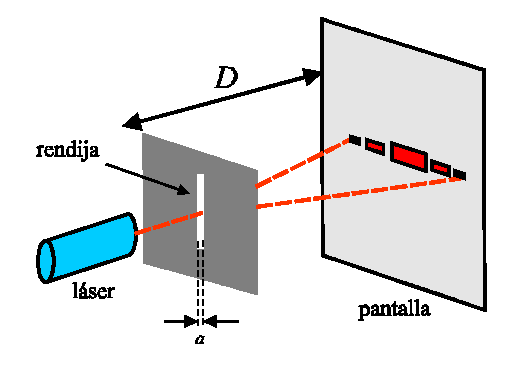
\includegraphics[width=8.5cm]{LG10--000.png}
    \caption{Esquema experimental del dispositivo propuesto para el 
    estudio de la difracci\'on de Fraunhoffer.}
    \label{fig:1}
\end{figure}

El protocolo experimental consiste entonces en desplazar el fotosensor a lo
largo de la figura de difracci\'on y registrar, para cada posici\'on, la
intensidad local de la luz que a \'el llega. El registro de los datos puede
realizarse mediante el sistema de adquisici\'on digital SensorDAQ, al cual
se encuentra conectado el sensor. El posicionador dispone de un tornillo 
microm\'etrico que permite medir la posici\'on del sensor sobre la figura
de difracci\'on. 

En estas condiciones:
\begin{itemize}
    \item Represente los resultados medidos en un gr\'afico $I(y)$, es decir,
        de intensidad observada en funci\'on de la posici\'on $y$ del
        fotosensor. Observe que la teor\'\i a predice un comportamiento dado
        por
        \begin{equation}
            I(y) = I_0 \left(\frac{\sin z(y)}{z(y)} \right)^2,
        \end{equation}
        siendo 
        \begin{equation*}
            z = \frac{\pi a}{\lambda} \sin \alpha(y).
        \end{equation*}
El \'angulo $\alpha$, que es funci\'on de $y$, mide la apertura angular de la 
figura de difracci\'on respecto del m\'aximo central, y verifica
\begin{equation}
    \tan \alpha(y) = \frac{y}{D},
\end{equation}
siendo $y$ la coodenada sobre la pantalla medida por el fotosensor. En este
caso, recuerde que si emple\'o el fot\'ometro para medir la intensidad, el
par\'ametro $D$ es la distancia desde el plano de la rendija hasta el elemento
sensible del instrumento.
\end{itemize}

\subsubsection*{Observaci\'on:}

El fotosensor satura a 3 V, lo que significa que cuando se lo ilumine con una
intensidad superior a la m\'axima, la lectura que dar\'a el instrumento ser\'a
siempre de 3 V. Dadas las caracter\'\i sticas del experimento, y siendo que 
deseamos observar los m\'aximos de intesidad, es posible que el m\'aximo de
orden cero resulte saturado. 


\nocite{Alonso1998,Jenkins2001,Hecht1986}
\bibliographystyle{unsrt} 
\bibliography{Bibliografia}

\end{document}
